\chapter{Ejercicio de seguimiento automático de carreteras con drones}\label{cap.followroad}
Una vez descrita la práctica anterior, se va a proceder a la descripción de la segunda práctica desarrollada para el elenco de prácticas de robótica de \textit{JdeRobot}. Esta práctica se llama \textit{Follow Road} y se va a explicar todo lo relacionado con su infraestructura, el nodo académico, la solución desarrollada y su experimentación.

\section{Enunciado}\label{sec.enunciado}
El objetivo de esta práctica, enfocado al estudiante, es el desarrollo de un algoritmo que dote de la inteligencia necesaria a un dron par que sea capaz de seguir una carretera. En este caso, se deben controlar la altitud, la velocidad y el giro del dron para poder realizar un correcto seguimiento de la carretera, por parte del dron. Esto supone un desafío para el alumno que deberá tener un control absoluto del robot en todo momento.

Para desarrollar la solución de esta práctica, el alumno debe enfrentarse a diversos problemas relacionados con la robótica. El primero de ellos es la visión, el alumno deberá realizar un procesado de imagen para filtrar los componentes que le interesen, en este caso, deberá filtrar la carretera. El segundo problema a abordar, es el control de movimiento del dron, en este caso, debe ser muy preciso porque se manejan alturas, además de giros y velocidades. El último problema vienen derivado de los dos anteriores y supone realizar un movimiento controlado y dinámico del dron, para ello el alumno debe procesar las imágenes y realizar un movimiento controlado del dron en función de la imagen procesada.

El desafío de esta práctica reside en la dificultad de mantener el dron estable en todo momento y adecuar sus movimientos al procesado de imagen que se realice. Esto supone la afrontación de los problemas anteriores de manera conjunta. Además, es necesario el desarrollo de un algoritmo robusto para evitar que el dron se estrelle o tenga un comportamiento anormal en casos extremos o en situaciones no previstas.

\section{Infraestructura}
En esta sección se abordarán los distintos elementos involucrados en la práctica (Figura \ref{fig.inf_fr}).

%\begin{figure}[H]
%  \begin{center}
%    \includegraphics[width=0.99\linewidth, height=5.5cm]{figures/prueba.png}
%		\caption{Infraestructura de Chrono}
%		\label{fig.inf_chrono}
%		\end{center}
%\end{figure}

\subsection{Arquitectura}
La arquitectura de esta práctica es distinta a las existentes hasta ahora. Esto se debe a la utilización de paquetes ROS en el dron. Para el funcionamiento del dron con ROS, es necesario un soporte en \textit{C++} llamado \textit{MAVLink}. \textit{MAVLink} es un protocolo de comunicación para vehículos autómatas. Este protocolo proporciona los mensajes para comunicarse con el dron. Apoyado en \textit{MAVLink}, se encuentra \textit{MavROS}. Se trata de un nodo de \textit{ROS} que realiza un conversión entre los \textit{topics} que se utilizan en \textit{ROS} para comunicarse con los robots y los mensajes de \textit{MAVLink} permitiendo, de esta manera, la comunicación de los vehículos autónomos con \textit{ROS}.Además, proporciona los \textit{plugins} y \textit{topics} finales del dron. Por encima de \textit{MavROS}, se han desarrollado unos drivers específicos para permitir la comunicación de la infraestructura \textit{JdeRobot} con \textit{ROS}, de esta manera, la plataforma \textit{JdeRobot} es integrable con \textit{ROS Kinetic}.
En cuanto al control de robot o vehículo autónomo, se ha utilizado el software libre \textit{Px4}. Se trata de un sistema de pilotaje automático de drones especialmente orientado a pilotaje fuera de la línea de visión del usuario. Este \textit{sofware} aporta la infraestructura básica del dron.
La infraestructura completa de esta práctica puede verse en la figura \ref{fig.arquitectura_fr}.

%\begin{figure}[H]
%  \begin{center}
%    \includegraphics[width=0.99\linewidth, height=5.5cm]{figures/prueba.png}
%		\caption{Arquitectura de Follow Road}
%		\label{fig.arquitectura_fr}
%		\end{center}
%\end{figure}

\subsubsection{Modelo dron ``Iris''}
Este modelo de dron ha sido escogido para la realización de esta práctica. Consta de un cuerpo principal, en el que va instalado el \textit{hardware}, cuatro rotores, una antena y dos cámaras. La inteligencia del dron viene dada por el sistema de pilotaje automático \textit{Px4}.

\begin{figure}[H]
	\begin{center}
	    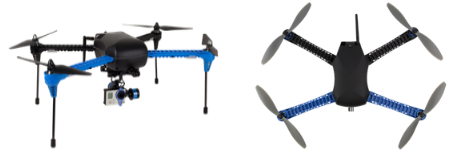
\includegraphics[width=0.98\textwidth]{figures/iris.png}
		\caption{Ilustraciones del dron ``Iris''}
		\label{fig.iris}
	\end{center}
\end{figure}

\subsubsection{Px4}
El piloto automático \textit{PX4}\footnote{\url{https://px4.io/}} es un sistema de piloto automático de código abierto orientado a aeronaves autónomas de bajo coste. Tanto el \textit{hardware} como el \textit{software} es \textit{open-source} y accesible gratuitamente bajo una licencia \textit{BSD}. Esta plataforma, derivó del proyecto \textit{PIXHWAK}\footnote{\url{http://pixhawk.org/}} que se centró, específicamente, en control de vuelo basado en visión. El \textit{software} incluido bajo \textit{Px4} incluye:
\begin{itemize}
    \item QGroundControl\footnote{\url{http://qgroundcontrol.com/}} y MAVLink para las comunicaciones con el dron.
    \item Mapas aéreos en 2D y 3D con soporte de Google Earth\footnote{\url{https://www.google.com/earth/}}.
    \item Puntos de control \textit{Drag-and-Drop}.
\end{itemize}

Esta infraestructura ha sido escogida por su compatibilidad de comunicaciones mediante el protocolo \textit{MAVLink}. Además, este sistema de autopilotaje tiene distintas características que lo convierten en la opción escogida para soporte de \textit{hardware} y \textit{software} de \textit{JdeRobot}:
\begin{itemize}
    \item Arquitectura modular y extensible.
    \item Código base simple para todos los vehículos.
    \item Desarrollado para conducción autónoma.
    \item Gran conjunto de periféricos compatibles.
    \item Modos de vuelo flexibles y potentes.
    \item Dispone de herramientas complementarias de desarrollo.
    \item Probado en modelos reales.
    \item Código \textit{open-source}.
\end{itemize}

Para esta práctica se ha utilizado la comunicación con el dron bajo los mensajes \textit{MAVLink}. De esta manera, \textit{Px4}, realiza la conversión de mensajes \textit{MAVLink} a comandos para el dron y viceversa.

\subsubsection{MAVLink}
El \textit{software} libre \textit{MAVLink}\footnote{\url{https://mavlink.io/en/}} (Micro Air Vehicle Link), es un protocolo de mensajes de comunicación en vehículos autónomos. Se ha diseñado como una librería de cálculo de referencia de encabezado simple. Fue lanzado a principios del año 2009 por Lorenz Meier bajo una licencia \textit{LGPL}\footnote{\url{https://en.wikipedia.org/wiki/GNU_Lesser_General_Public_License}}.

Los mensajes están definidos con ficheros \textit{XML}. Cada fichero \textit{XML} define un conjunto de mensajes admitidos por un sistema \textit{MAVLink} particular o dialecto.

\subsubsection{MavROS}
El nodo de \textit{ROS}, \textit{MavROS}\footnote{\url{http://wiki.ros.org/mavros}}\footnote{\url{http://ardupilot.org/dev/docs/ros.html}}, es un paquete que proporciona un controlador de comunicación para varios pilotos automáticos con el protocolo de comunicación \textit{MAVLink} y un puente \textit{UDP MAVLink} para estaciones de control terrestre.

\textit{MavROS} esta formado por cuatro componentes:
\begin{itemize}
    \item Nodos \textit{MavROS}. Estos nodos están formados por \textit{topics} de suscripción, \textit{topics} de publicación y parámetros de configuración.
    \item Puente \textit{GCS}. Es la conexión de \textit{MavROS} con el protocolo de mensajes \textit{MAVLink}.
    \item Lanzador de eventos. Comprueba el estado de los eventos producidos por los \textit{topics}.
    \item \textit{Plugins}. \textit{MavROS} proporciona un gran número de \textit{topics} a los que poder suscribirte para recibir información del estado del dron o para publicar comandos de control del dron. A este conjunto de \textit{plugins} se accede gracias a los \textit{topics}. Cada \textit{plugins} contiene distintos \textit{topics} o tipos de mensajes distintos con los que enviar o recibir información del \textit{plugin}. Una vez recibida esta información, el \textit{plugin} realiza una transformación de mensajes \textit{MAVLink} a \textit{topics} de \textit{ROS} y viceversa.  Los \textit{topics} ofrecidos por los \textit{plugins} de \textit{MavROS} son más de cien pero, para el control del dron en \textit{JdeRobot}, se han utilizado los siguientes:
        \item /mavros/cmd/arming: para armar el dron.
        \item /mavros/global\_position/global: para conocer la posición gps del dron y realizar el despegue.
        \item /mavros/cmd/takeoff: para despegar el dron.
        \item /mavros/cmd/land: para aterrizar el dron.
        \item /mavros/set/mode: para cambiar el dron entre sus distintos modos.
            \item Auto\_RTL: Modo automático. Se utiliza para despegar y aterrizar.
            \item Offboard: Modo manual. Se utiliza para controlar el dron.
        \item /mavros/setpoint\_raw/local: para controlar el movimiento del dron. Permite enviar información de posición, altura, velocidad, aceleración y giro. 
        \item /mavros/local\_position/odom: para recibir la odometría del dron.
        \item /iris\_fpv\_cam/cam\_XXXXX/image\_raw: aunque no se trata de un \textit{topic} proporcionado por \textit{MavROS}, utiliza \textit{ROS} para recibir información de las cámaras, por lo que es integrable con \textit{MavROS}.
\end{itemize}

\subsubsection{Drivers}
Para realizar las conexiones a los \textit{topics} ofrecidos por \textit{MavROS}, se han desarrollado unos drivers, específicos para la infraestructura de \textit{JdeRobot}. Para ello se han desarrollado un total de seis ficheros con código en \textit{Python} que dotan de la infraestructura necesaria, al nodo académico, para comunicarse con el dron.

\begin{itemize}
    \item En el fichero \textit{\_\_init\_\_.py}, se establecen las cabeceras de las funciones principales de interconexión y las conexiones de los \textit{topics}.
    \item En el fichero \textit{camera.py}, se han desarrollado las funciones necesarias para recoger las imágenes captadas por las cámaras integradas en el dron.
    \item En el fichero \textit{cmdvel.py}, se incorporan las funciones necesarias para enviar los comandos de velocidad al plugin de \textit{MavROS}.
    \item En el fichero \textit{extra.py}, se han desarrollado las funciones para controlar el despegue y aterrizaje del dron.
    \item En el fichero \textit{pose3d.py}, están las funciones para recoger la información sobre la odometría del dron.
    \item En el fichero \textit{threadPublisher.py}, está la función de creación de la hebra para las comunicaciones de las hebras de publicación de \textit{topics}.
\end{itemize}


\subsubsection{Sensores y actuadores}
Una vez descritos los componentes de comunicación con el dron, se va a explicar los componentes que forman el modelo del dron. Estos componentes dotan al dron de la estructura y movilidad necesaria para su funcionamiento.

\paragraph{Cámara}
La cámara proporciona al dron visión del escenario en el que se encuentra. Es necesaria para dotar al dron de una interfaz sobre la que basar su inteligencia. En esta práctica son necesarias dos cámaras, una frontal y otra ventral para tener un visión del entorno tanto en la parte delantera del dron, para evitar obstáculos, como inferior para poder visualizar correctamente la carretera.

El \textit{plugin} de la cámara es proporcionado por \textit{ROS}. Este \textit{plugin} proporciona el código necesario para conectar una cámara mediante USB con una velocidad de refresco de 30 imágenes por segundo  con una longitud focal de 277 milímetros. Con estas características, el dron puede recoger imágenes a una velocidad lo suficientemente rápida y a una distancia apropiada, para procesar las imágenes y conseguir evitar los obstáculos con suficiente antelación.

Las imágenes captadas por la cámara son recogidas por el nodo académico gracias a su interfaz gráfica y mediante un API simple. De esta manera se pueden visualizar las imágenes de las cámaras en la interfaz gráfica del nodo académico, así como su procesado.

\paragraph{Sensor Odométrico}
Con este sensor, el dron es capaz de conocer su posición. Este sistema se implementa gracias al GPS que incorpora el dron y le permite conocer su latitud y longitud en el escenario en el que se encuentre. \textit{MavROS} incorpora \textit{topics} para conocer esta posición. El \textit{topic} utilizado para estimar esta posición ofrece la posición del dron en coordenadas relativas al lugar de despegue del dron. Esta funcionalidad viene soportada en el \textit{plugin setpoint\_position}.

\paragraph{Rotores}
El dron está formado por cuatro rotores que permite su movimiento. Para el control de estos rotores, se incorpora un \textit{plugin} de control de rotor por cada uno de los rotores del dron. Este \textit{plugin} es proporcionado por \textit{Px4} y es de \textit{ROS}. Sin embargo, el \textit{plugin} que se utiliza para mover el dron es proporcionado por \textit{MavROS} bajo el nombre \textit{setpoint\_raw} al que se accede con el \textit{topic /mavros/setpoint\_raw/local}. 

\paragraph{Escenario de Gazebo}
Para esta práctica se ha actualizado el escenario inicial del que disponía la práctica y se han arreglado problemas que presentaba relacionados con la visualización del suelo, un nuevo modelo de casa y la incorporación del modelo del dron nuevo. El aspecto del escenario puede verse en la figura \ref{fig.mundo_fr}.

\begin{figure}[H]
  \begin{center}
    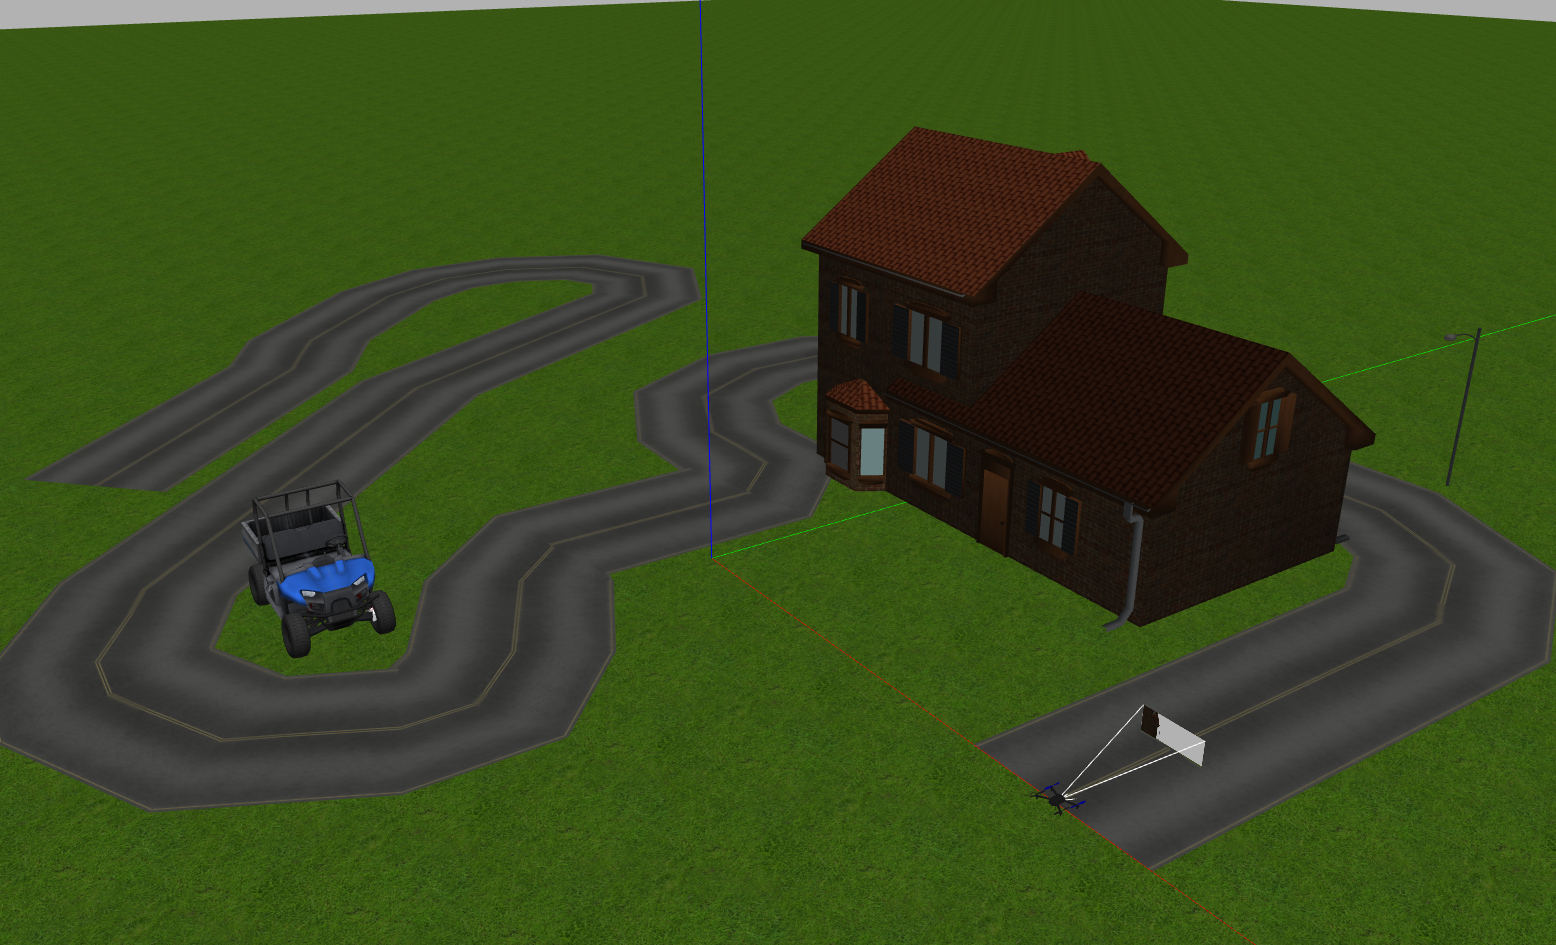
\includegraphics[width=0.9\linewidth]{figures/mundo_fr.png}
		\caption{Escenario de Follow Road}
		\label{fig.mundo_fr}
		\end{center}
\end{figure}

\paragraph{Ficheros de configuración} \label{sec.launch_fr}
Para la incorporación del modelo del circuito y del robot, es necesario la creación de un modelo de configuración que importe en \textit{Gazebo} los elementos de los que consta el escenario y su localización. Este fichero tiene la extensión \textit{.world} y \textit{Gazebo} es capaz de leerlo y mostrar el escenario al iniciarse.
El código del fichero es el siguiente:

\lstset{language=XML, breaklines=true, basicstyle=\footnotesize}
\begin{lstlisting}[frame=single]
<?xml version="1.0" ?>
<sdf version="1.5">
  <world name="default">
    <scene>
      <grid>false</grid>
    </scene>
    <!-- A global light source -->
    <include>
      <uri>model://sun</uri>
    </include>
    <include>
      <uri>model://grass_plane</uri>
    </include>

    <include>
      <uri>model://house_4</uri>
      <pose>1 6.43 0 0 0 0</pose>
    </include>
    <include>
      <uri>model://polaris_ranger_ev</uri>
      <pose>-1.48 -6 0.1 0 0 0</pose>
      <static>true</static>
    </include>
    <include>
      <uri>model://lamp_post</uri>
      <pose>5 13 0 0 0 0</pose>
    </include>
    <include>
      <uri>model://lamp_post</uri>
      <pose>-4 13 0 0 0 0</pose>
    </include>
    <include>
      <uri>model://iris_fpv_cam</uri>
      <pose>8 0 0.3 0 0 1.57</pose>
    </include>
    <road name="my_road">
      <width>3</width>

      <point>8 0 0.01</point>
      <point>8 3 0.01</point>
      <point>8 8 0.01</point>
      <point>7 10 0.01</point>
      <point>5 11 0.01</point>
      <point>-5 11 0.01</point>
      <point>-7 10 0.01</point>
      <point>-8 8 0.01</point>
      <point>-8 6 0.01</point>
      <point>-7 4 0.01</point>
      <point>-5 3 0.01</point>
      <point>-3 3 0.01</point>
      <point>-2 2 0.01</point>
      <point>-2 -2 0.01</point>
      <point>-1 -3 0.01</point>

      <point>1 -4 0.01</point>
      <point>2 -5 0.01</point>

      <point>2 -6 0.01</point>
      <point>1 -8 0.01</point>
      <point>-1 -9 0.01</point>
      <point>-2 -9 0.01</point>
      <point>-4 -8 0.01</point>

      <point>-11 -1 0.01</point>
      <point>-14 5 0.01</point>

      <point>-15 7 0.01</point>
      <point>-17 8 0.01</point>
      <point>-19 7 0.01</point>

      <point>-20 5 0.01</point>
      <point>-20 3 0.01</point>
      <point>-19 1 0.01</point>
      <point>-17 -1 0.01</point>

      <point>-16 -2 0.01</point>
      <point>-14 -3 0.01</point>
      <point>-9 -8 0.01</point>
    </road>
  </world>
</sdf>
\end{lstlisting}

Además de este fichero de configuración, es necesario un fichero complementario que importe los \textit{plugins y drivers} de ROS-Kinetic. Este tipo de fichero tienen la extensión \textit{.launch}. En este fichero se pasan a \textit{Gazebo} argumentos como el nombre del fichero de configuración con el escenario, establecer el tiempo que se va a utilizar en el escenario, la posible implementación de un GUI y otras opciones de depuración.
El fichero es el siguiente:

\lstset{language=XML, breaklines=true, basicstyle=\footnotesize}
\begin{lstlisting}[frame=single]
<?xml version="1.0" encoding="UTF-8"?>
<launch>
  <!-- We resume the logic in empty_world.launch, changing only the name of the world to be launched -->
  <include file="$(find gazebo_ros)/launch/empty_world.launch">
    <arg name="world_name" value="road_drone_textures_ROS.world"/> <!-- Note: the world_name is with respect to GAZEBO_RESOURCE_PATH environmental variable -->
    <arg name="paused" value="false"/>
    <arg name="use_sim_time" value="true"/>
    <arg name="gui" value="true"/>
    <arg name="headless" value="false"/>
    <arg name="debug" value="false"/>
    <arg name="verbose" default="true"/>
  </include>

  <arg name="fcu_url" default="udp://:14540@127.0.0.1:14540" />
	<arg name="gcs_url" default="" />
	<arg name="tgt_system" default="1" />
	<arg name="tgt_component" default="1" />
	<arg name="log_output" default="screen" />
	<arg name="fcu_protocol" default="v2.0" />
	<arg name="respawn_mavros" default="false" />

	<include file="$(find mavros)/launch/node.launch">
		<arg name="pluginlists_yaml" value="$(find mavros)/launch/px4_pluginlists.yaml" />
		<arg name="config_yaml" value="$(find mavros)/launch/px4_config.yaml" />

		<arg name="fcu_url" value="$(arg fcu_url)" />
		<arg name="gcs_url" value="$(arg gcs_url)" />
		<arg name="tgt_system" value="$(arg tgt_system)" />
		<arg name="tgt_component" value="$(arg tgt_component)" />
		<arg name="log_output" value="$(arg log_output)" />
		<arg name="fcu_protocol" value="$(arg fcu_protocol)" />
		<arg name="respawn_mavros" default="$(arg respawn_mavros)" />
	</include>

  <node pkg="mavros" type="px4.sh"  name="px4" output="screen"/>
</launch>
\end{lstlisting}

\subsection{Arquitectura software}
Esta práctica tiene tes hilos de ejecución para aliviar la carga computacional de la práctica De esta manera se aumenta la velocidad  la que puede trabajar el simulador \textit{Gazebo}.

\begin{itemize}
	\item Hilo de sensores: este hilo se encarga de la actualización de los datos de los sensores del robot. Este hilo se comunica con \textit{Gazebo} para recoger datos de la odometría y la cámara y entregárselos al nodo académico.
	\item Hilo de la interfaz gráfica del usuario (GUI): este hilo se encarga del refresco del GUI de la práctica. En esta práctica tiene una carga computacional elevada dado se encarga de refrescar las imágenes obtenidas por la cámaras, el procesamiento visual sobre esa imagen que ha realizado el alumno, un mapa del circuito con la posición actualizada del robot y del robot fantasma a vencer, y una lectura controlada de tiempos para sincronizar ambos coches.
	\item Hilo de actuadores: este hilo se encarga de enviar la información del nodo académico al dron. Se conecta con \textit{Gazebo} para enviar las órdenes de movimiento.
\end{itemize}

\subsubsection{Interfaz gráfica}
La interfaz gráfica del usuario (GUI), se utiliza para representar información relacionada con los sensores del robot. Esta información es muy útil para la depuración del algoritmo del estudiante ya que permite la visualización de las publicaciones que realiza el algoritmo al robot.

Esta GUI (Figura \ref{fig.guifr}) está formada por tres conjuntos \textit{widgets}, uno para el visionado del de las imágenes, otro para su control y otro para el teleoperador.

\begin{figure}[H]
  \begin{center}
    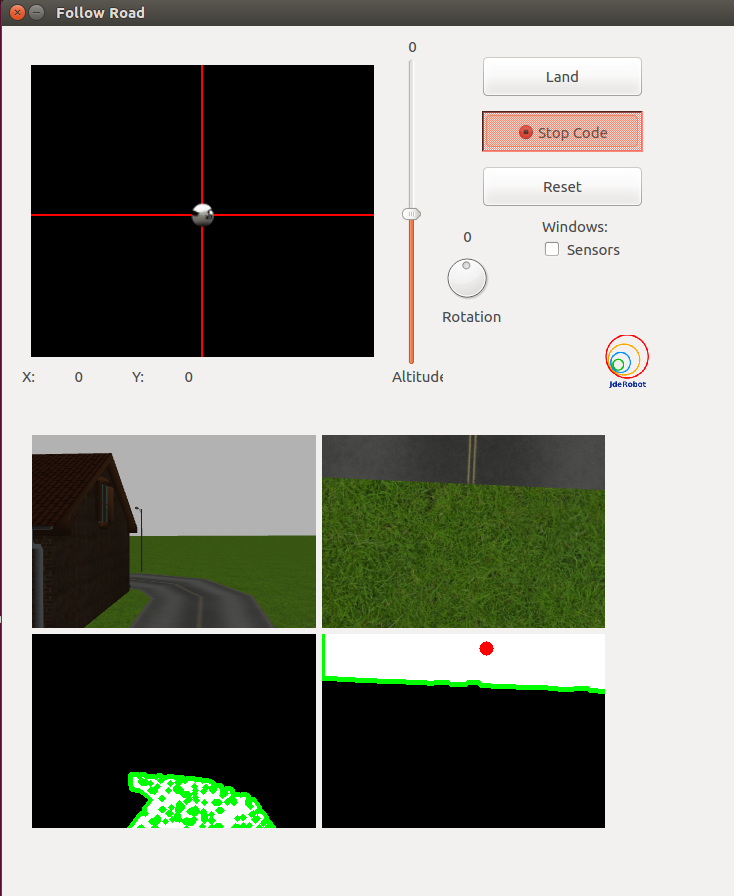
\includegraphics[width=7cm,height=10cm,\textwidth]{figures/GUI_fr.png}
		\caption{Interfaz Gráfica Folow Road}
		\label{fig.guifr}
		\end{center}
\end{figure}

El \textit{widget} del teleoperador se utiliza para controlar el dron una vez ha despegado. De esta manera se puede comprobar que las conexiones del dron están correctamente realizadas.

El conjunto \textit{widgets} destinados al control del dron se dividen en tres subconjuntos:
\begin{itemize}
    \item Control de altitud y rotación.
    \item wirdgets de estabilización.
    \item Botón de despegue/aterrizaje, botón de ejecución y parada del algoritmo de solución y botón de reinicio del puntero del teleoperador.
\end{itemize}
Con estos \textit{widgets} se puede controlar el dron de manera manual o mediante la programación de la inteligencia del dron en el fichero de solución.

El \textit{widget} de visionado del dron incorpora cuatro pantallas. Las pantallas superiores reflejan las imágenes recogidas por las cámaras del dron y las pantallas inferiores muestran el procesado de las imágenes realizado en el algoritmo del solución del alumno. Este último \textit{widget} es muy útil para depurar el algoritmo del alumno ya que puede verse, fácilmente, el procesado que se ha realizado de la imagen.

\section{Nodo Académico}
Una vez explicado toda la infraestructura circundante al nodo académico de la práctica, se va a explicar la infraestructura del propio nodo. Esta formado por:

\begin{itemize}
    \item Fichero principal.
    \item Fichero de solución
    \item GUI. Directorio con todos los ficheros para el funcionamiento del GUI.
\end{itemize}

El fichero principal es el código que va a ejecutarse para lanzar el nodo académico de la práctica. En él se especifican las conexiones con los \textit{topics} que se van a establecer, así como la inizalización del GUI.

En el fichero de solución, hay un conjunto de funciones que aportan la funcionalidad de la práctica, como comenzar, parar, recoger imagen, así como las que desarrolle el alumno y el propio código con la solución de referencia.

\section{Solución de referencia}
Para esta práctica se han desarrollado dos soluciones de referencia. La primera solución se ha desarrollado para la práctica inicial que no contaba con soporte para \textit{ROS} y se realizaba con \textit{drivers ICE}. La segunda solución desarrollada es compatible con \textit{ROS}. Ambas soluciones han sido desarrolladas íntegramente.

\subsection{Procesamiento de imagen}
El procesamiento de las imágenes programado se ha realizado en función del contorno del filtrado. Para ello se comienza con la recogida de las imágenes captadas por la cámara:

\lstset{language=Python, breaklines=true, basicstyle=\footnotesize}
\begin{lstlisting}[frame=single]
input_imageV = self.drone.getImageVentral().data
input_imageF = self.drone.getImageFrontal().data
\end{lstlisting}

Con esta instrucción, es posible visualizar las imágenes en el GUI.

Tras obtener las imágenes frontal y ventral de la cámara, hay que transformarla a una imagen HSV\footnote{\url{https://es.wikipedia.org/wiki/Modelo_de_color_HSV}} para poder seleccionar el color de la carretera:

\lstset{language=Python, breaklines=true, basicstyle=\footnotesize}
\begin{lstlisting}[frame=single]
image_HSV_V = cv2.cvtColor(input_imageV, cv2.COLOR_RGB2HSV)
image_HSV_F = cv2.cvtColor(input_imageF, cv2.COLOR_RGB2HSV)
\end{lstlisting}

Tras obtener la imagen HSV, podemos seleccionar el rango de valores que componen color de la carretera como un array con la intensidad mínima y máxima del color.

\lstset{language=Python, breaklines=true, basicstyle=\footnotesize}
\begin{lstlisting}[frame=single]
value_min_HSV = np.array([20, 0, 0])
value_max_HSV = np.array([100, 130, 130])
\end{lstlisting}

Con esos valores realizamos un filtrado de la imagen para obtener la carretera, exclusivamente:

\lstset{language=Python, breaklines=true, basicstyle=\footnotesize}
\begin{lstlisting}[frame=single]
image_HSV_filtered_V = cv2.inRange(image_HSV_V, value_min_HSV, value_max_HSV)
image_HSV_filtered_F = cv2.inRange(image_HSV_F, value_min_HSV, value_max_HSV)
\end{lstlisting}

Para reducir el ruido que contiene la la imagen sobre los colores filtrados es necesario aplicar técnicas de reducción de ruido. Para ello hemos realizado una apertura y un cierre de la imagen:

\lstset{language=Python, breaklines=true, basicstyle=\footnotesize}
\begin{lstlisting}[frame=single]
opening_V = cv2.morphologyEx(image_HSV_filtered_V, cv2.MORPH_OPEN, np.ones((5,5),np.uint8))
closing_V = cv2.morphologyEx(opening_V, cv2.MORPH_CLOSE, np.ones((10,10),np.uint8))
\end{lstlisting}

Para el caso de la imagen frontal, hemos realizado una técnica de apertura, solamente, con lo que se obtendrá más ruido que con la combinación anterior:

\lstset{language=Python, breaklines=true, basicstyle=\footnotesize}
\begin{lstlisting}[frame=single]
opening_F = cv2.morphologyEx(image_HSV_filtered_F, cv2.MORPH_OPEN, np.ones((5,5),np.uint8))
\end{lstlisting}

Una vez tenemos el filtro, lo utilizamos como una máscara para realizar el filtrado de la imagen y obtiener la imagen filtrada en formato binario, con el rango de colores que pasan el filtro en blanco:

\lstset{language=Python, breaklines=true, basicstyle=\footnotesize}
\begin{lstlisting}[frame=single]
image_HSV_filtered_Mask_V = np.dstack((closing_V, closing_V, closing_V))
image_HSV_filtered_Mask_F = np.dstack((opening_F, opening_F, opening_F))
\end{lstlisting}

Una vez realizado el filtrado, es necesario convertir la imagen a escala de grises para poder dibujar el contorno de la sección filtrada:

\lstset{language=Python, breaklines=true, basicstyle=\footnotesize}
\begin{lstlisting}[frame=single]
imgray_V = cv2.cvtColor(image_HSV_filtered_Mask_V, cv2.COLOR_BGR2GRAY)
ret_V, thresh_V = cv2.threshold(imgray_V, 127, 255, 0)
_, contours_V, hierarchy_V = cv2.findContours(thresh_V, cv2.RETR_TREE, cv2.CHAIN_APPROX_SIMPLE)
cv2.drawContours(image_HSV_filtered_Mask_V, contours_V, -1, (0,255,0), 3)

imgray_F = cv2.cvtColor(image_HSV_filtered_Mask_F, cv2.COLOR_BGR2GRAY)
ret_F, thresh_F = cv2.threshold(imgray_F, 127, 255, 0)
_, contours_F, hierarchy_F = cv2.findContours(thresh_F, cv2.RETR_TREE, cv2.CHAIN_APPROX_SIMPLE)
cv2.drawContours(image_HSV_filtered_Mask_F, contours_F, -1, (0,255,0), 3)
\end{lstlisting}

Tras dibujar el contorno de la sección, es necesaria una comprobación del filtrado de la imagen para evitar errores en la ejecución. El siguiente algoritmo comprueba si se ha recogido alguna imagen, si hay alguna zona que ha pasado el filtro y se hay más de una sección filtrada (para el caso en que se detecten varias carreteras):

\lstset{language=Python, breaklines=true, basicstyle=\footnotesize}
\begin{lstlisting}[frame=single]
area = []
for pic, contour in enumerate(contours_V):
    area.append(cv2.contourArea(contour))

if len(area) > 1:
    if area[0] < area[1]:
        M = cv2.moments(contours_V[1])
    else:
        M = cv2.moments(contours_V[0])

else:
    try:
        M = cv2.moments(contours_V[0])
    except IndexError:
        self.drone.sendCMDVel(0,0.3,0,0)
        M = cv2.moments(0)
\end{lstlisting}

Si la comprobación es exitosa, se extraen las coordenadas del centro de la sección filtrada:

\lstset{language=Python, breaklines=true, basicstyle=\footnotesize}
\begin{lstlisting}[frame=single]
if int(M['m00']) != 0:
    cx = int(M['m10']/M['m00'])
    cy = int(M['m01']/M['m00'])
\end{lstlisting}

Se dibuja un punto rojo para saber el centro de la sección filtrada, punto el cual seguirá el dron:

\lstset{language=Python, breaklines=true, basicstyle=\footnotesize}
\begin{lstlisting}[frame=single]
cv2.circle(image_HSV_filtered_Mask_V, (cx, cy), 7, np.array([255, 0, 0]), -1)
\end{lstlisting}

Para visualizar en el GUI el procesado de las imágenes se utilizan las siguientes instrucciones:

\lstset{language=Python, breaklines=true, basicstyle=\footnotesize}
\begin{lstlisting}[frame=single]
self.setImageFilteredVentral(image_HSV_filtered_Mask_V)
self.setImageFilteredFrontal(image_HSV_filtered_Mask_F)
\end{lstlisting}

\subsection{Control de movimiento}
Una vez procesada la imagen, es posible controlar el dron con el punto del centro de la sección obtenido. De esta manera, el dron se limitará a seguir dicho punto, adecuando sus movimientos hacia el mismo.

\lstset{language=Python, breaklines=true, basicstyle=\footnotesize}
\begin{lstlisting}[frame=single]
if cy > 120:
    self.drone.sendCMDVel(0,0.3,0,0.2)
    print("Turning")
elif cx < 20:
    print("Detected two roads")
    self.drone.sendCMDVel(0,0.3,0.1,0.0)
else:
    self.drone.sendCMDVel(0,0.3,0,0.0)

print("cx: " + str(cx) + " cy: " + str(cy))
self.yaw = int(cx)
\end{lstlisting}

\section{Experimentación}
La optimización de los algoritmos anteriores ha sido posible gracias a la realización de
diversos experimentos. Estos experimentos han hecho salir a la luz errores en el algoritmo
desarrollado que han sido subsanados.
Además se han realizado experimentos globales donde se ha testeado la práctica en su
totalidad, nodo académico, infraestructura de la práctica y solución desarrollada.

\subsection{Ejecución típica}
Se ha preparado un documento \textit{README.md}, incluido en la infraestructura de la práctica, que sirve de guía al alumno a la hora de ejecutar la práctica. En él se incluye información acerca de su ejecución, la API de los sensores y actuadores de ROS e, incluso, un vídeo demostrativo con una ejecución.

Para ejecutar al práctica, es necesario lanzar en una terminal el fichero de configuración de ROS, llamado \textit{follow\_road.launch}, descrito en la sección \ref{sec.launch_fr}. Para lanzar el fichero hay que ejecutar el siguiente comando:

\lstset{language=bash, breaklines=true, basicstyle=\footnotesize}
\begin{lstlisting}[frame=single]
roslaunch follow_road.launch
\end{lstlisting}

Una vez lanzado el comando en la terminal, se abrirá el simulador \textit{Gazebo} con el escenario del circuito (Figura \ref{fig.circuito}).

\begin{figure}[H]
  \begin{center}
    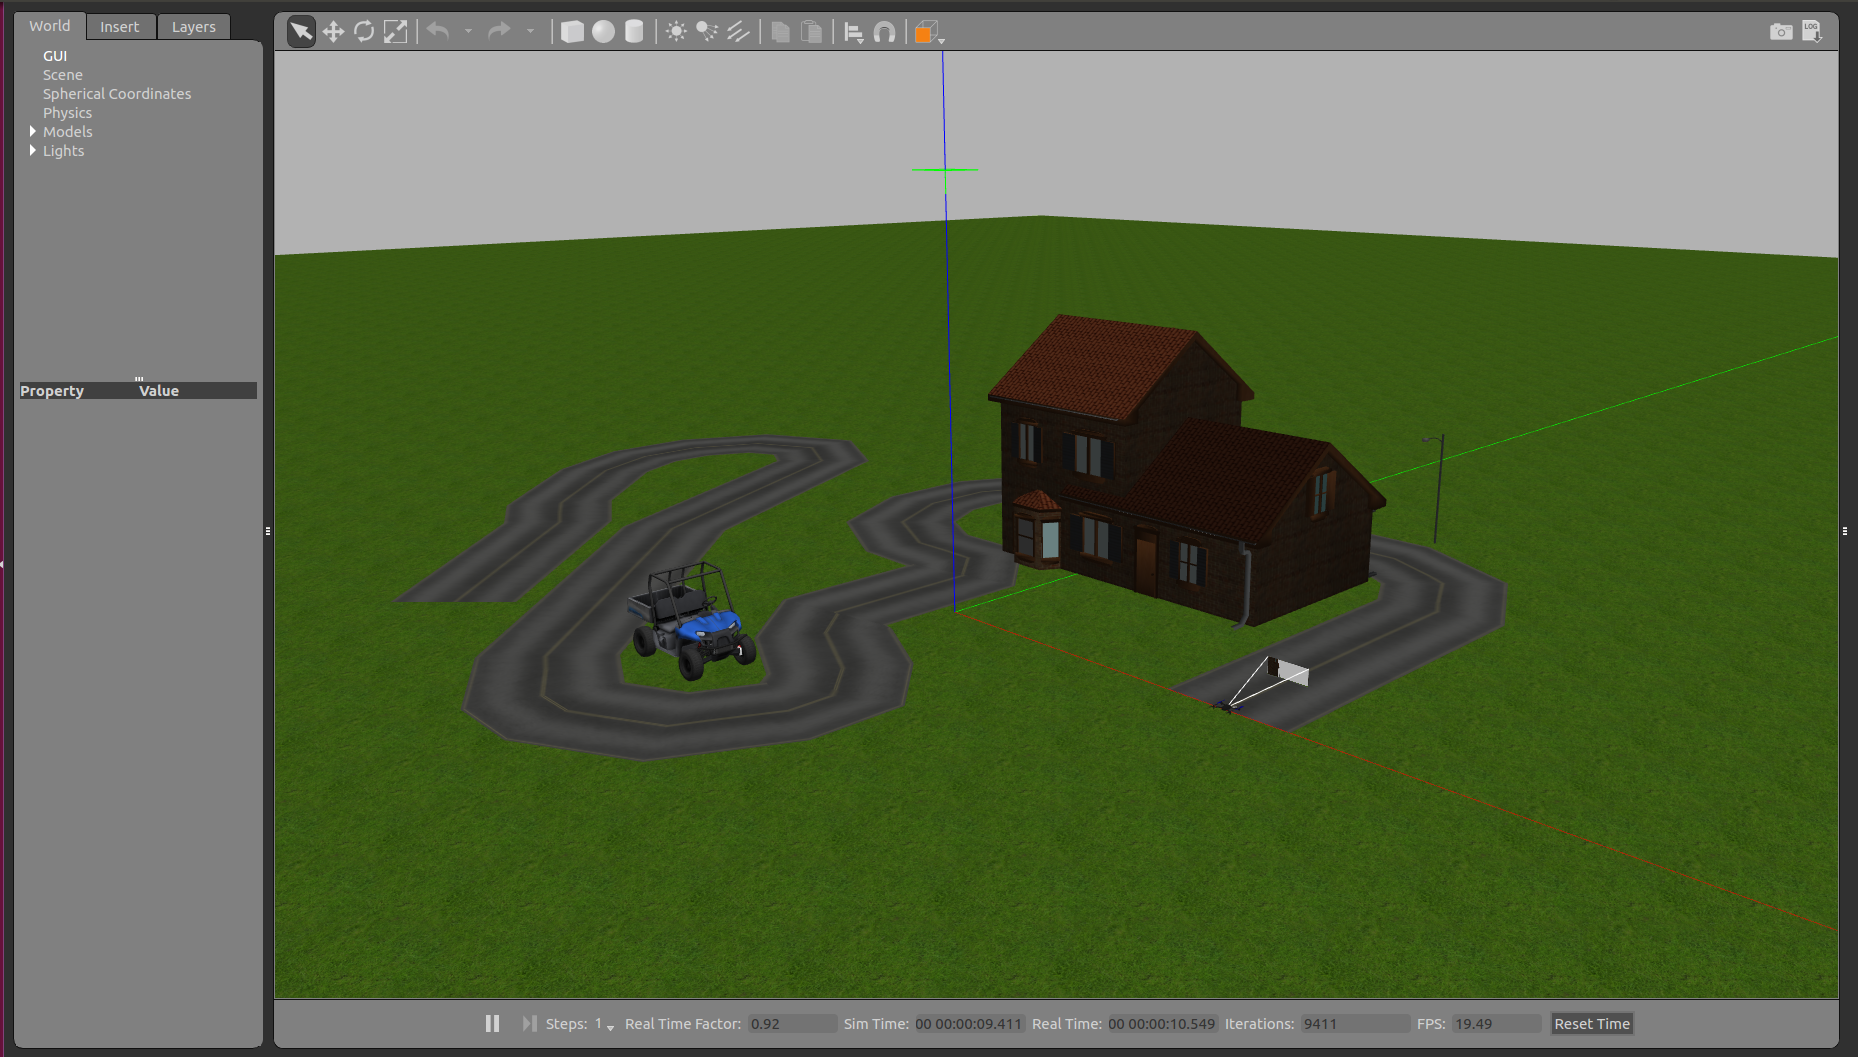
\includegraphics[width=0.98\textwidth]{figures/roslaunch_fr.png}
		\caption{Inicialización ROS y Gazebo}
		\label{fig.roslaunchfr}
		\end{center}
\end{figure}

Para iniciar el componente académico, será necesario ejecutar otro comando en una terminal distinta:

\lstset{language=bash, breaklines=true, basicstyle=\footnotesize}
\begin{lstlisting}[frame=single]
cd ~/Academy/exercises/follow\_road
python2 follow\_road.py
\end{lstlisting}

Una vez ejecutado el comando, el componente académico enlazará los sensores y actuadores proporcionados por \textit{ROS-Kinetic} mediante el fichero de configuración lanzado previamente a la variable \textit{self.drone} que contiene las variables:

\begin{itemize}
    \item self.cameraVentral
    \item self.cameraFrontal
    \item self.pose3d
    \item self.cmdvel
    \item self.extra
\end{itemize}

Con la variable \textit{self.drone}, el nodo académico se comunica con los \textit{drivers} de \textit{ROS-Kinetic}.
Además de realizar la conexión con los sensores y actuadores, al ejecutar la instrucción, nos aparecerá la interfaz gráfica de usuario (GUI) en la que se podrá visualizar las imágenes recogidas por la cámara, los botones de control y el teleoperador (Figura \ref{fig.inaGfr}).

\begin{figure}[H]
  \begin{center}
    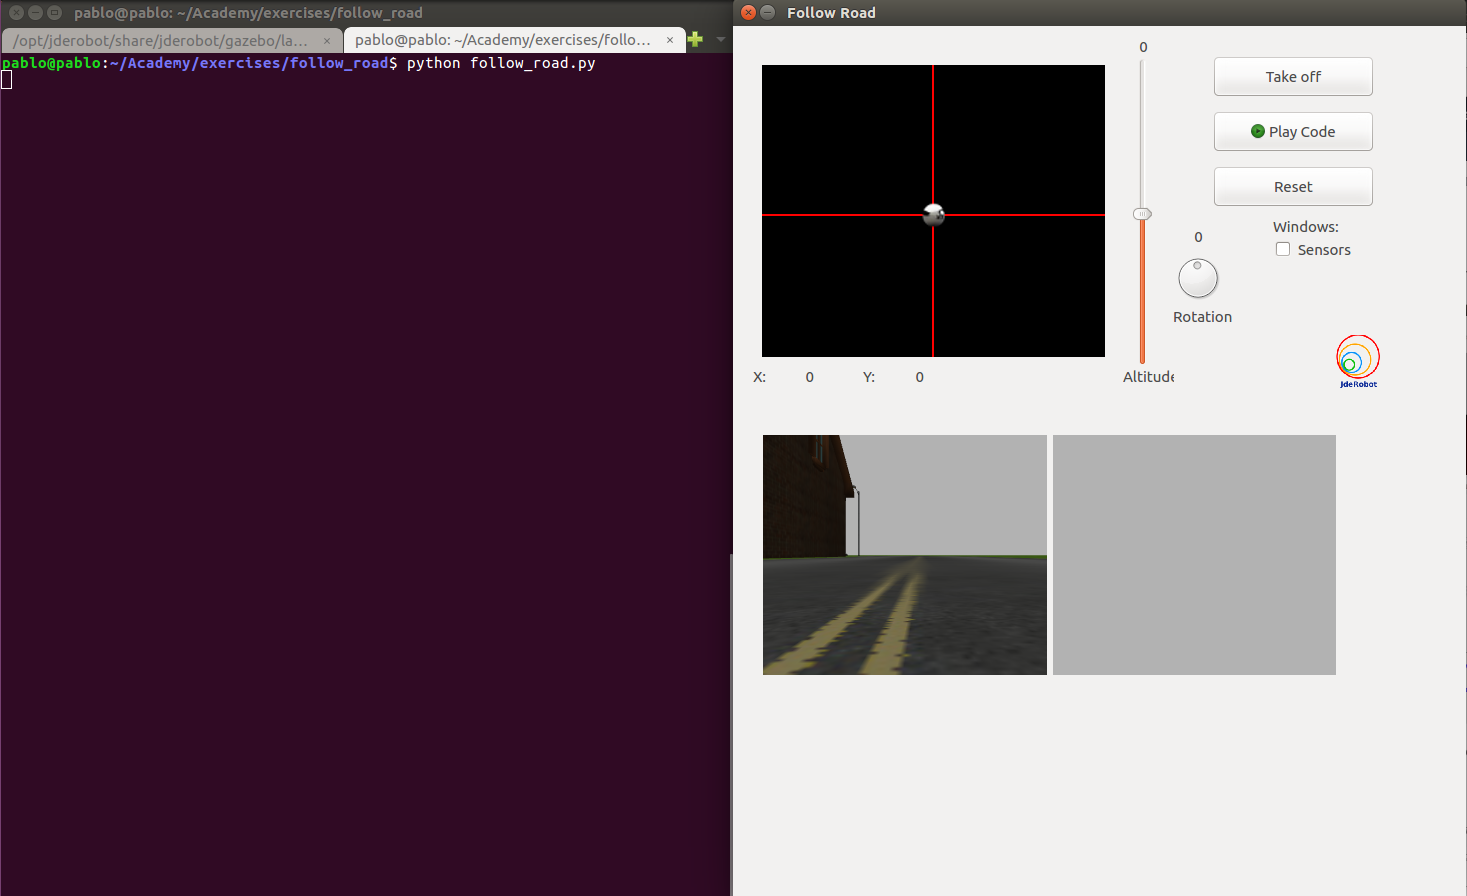
\includegraphics[width=0.98\textwidth]{figures/init_na_fr.png}
		\caption{Inicialización del nodo académico y el GUI}
		\label{fig.inaGfr}
		\end{center}
\end{figure}

Una vez inicializados los \textit{drivers de ROS-Kinetic}, el escenario en el simulador y el nodo académico, con su GUI, se puede iniciar el algoritmo desarrollado por el alumno pulsando sobre el botón ``Play Code''. De esta manera, la lógica programada podrá ser visualizada tanto en el GUI, como en el simulador.

\subsection{Ejecución estática}
En el caso en el que el alumno no programe el control de movimiento en su algoritmo, es posible ejecutar el código de igual manera. Esto es útil para depurar el algoritmo de procesamiento de imagen. 

El alumno tiene dos opciones en este aspecto. La primera consiste en dejar el robot inmóvil y ver el procesamiento realizado en la ventana para la imagen procesada del GUI. 

\begin{figure}[H]
  \begin{center}
    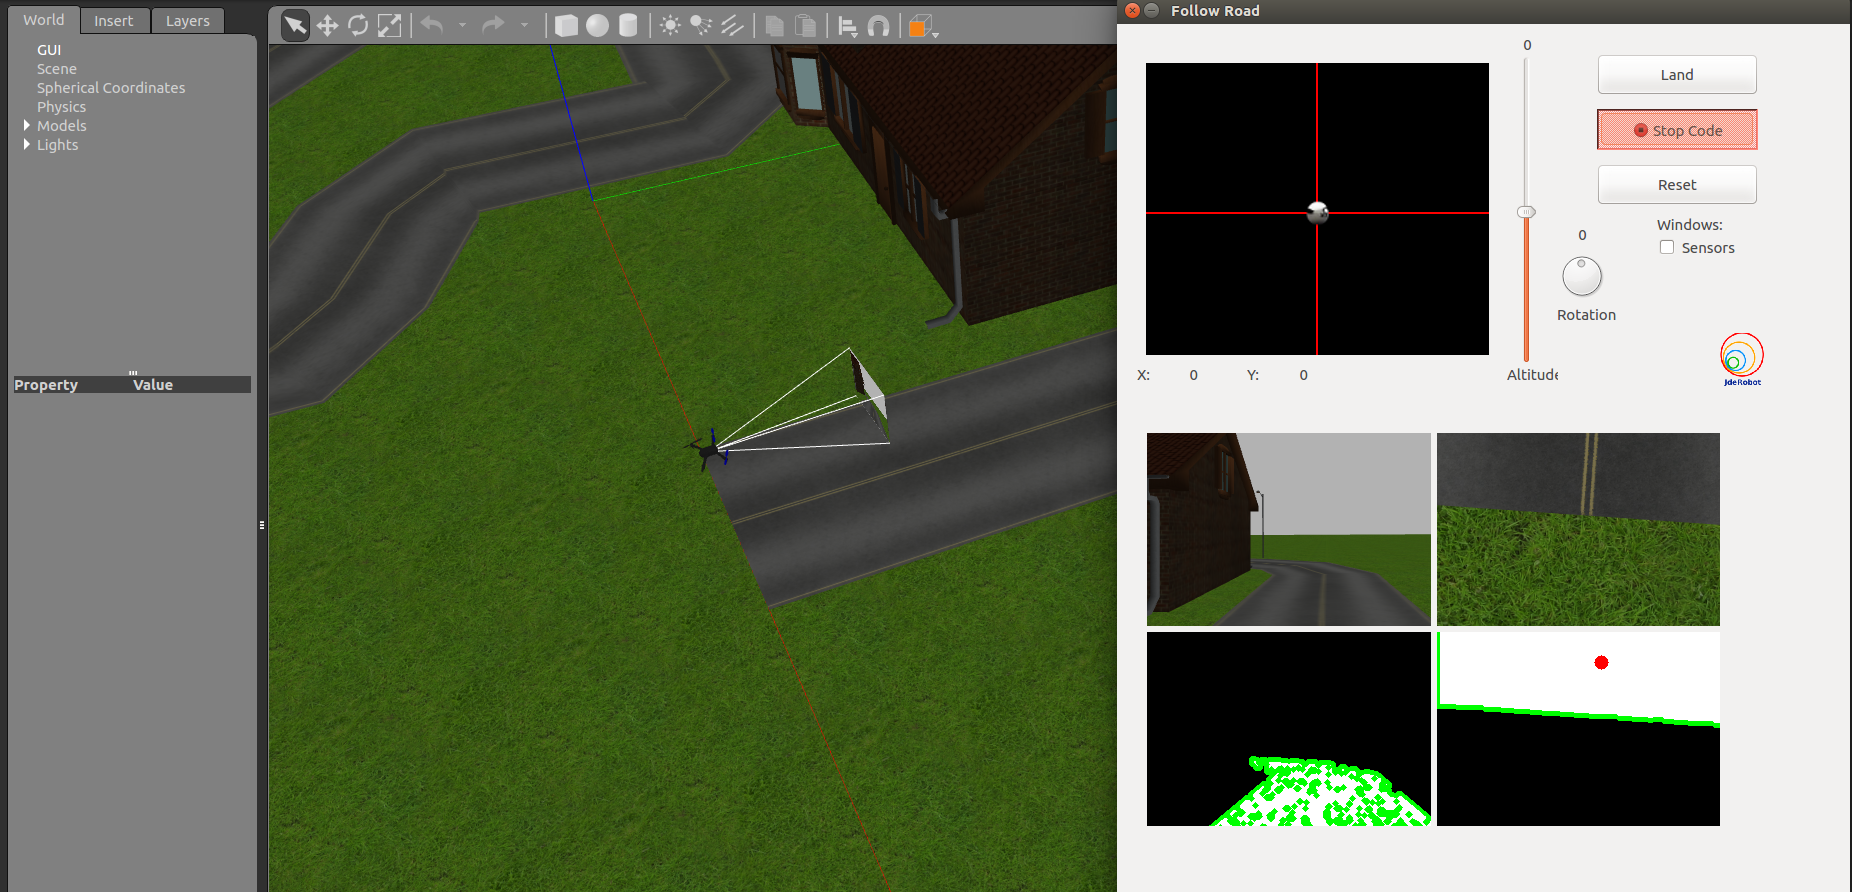
\includegraphics[width=0.98\textwidth]{figures/ejec_estat_fr.png}
		\caption{Ejecución estática de la práctica}
		\label{fig.eefr}
		\end{center}
\end{figure}

Otra opción, una vez haya superado esa primera prueba, es utilizar el teleoperador para mover el dron y visualizar el filtrado en movimiento.

\begin{figure}[H]
  \begin{center}
    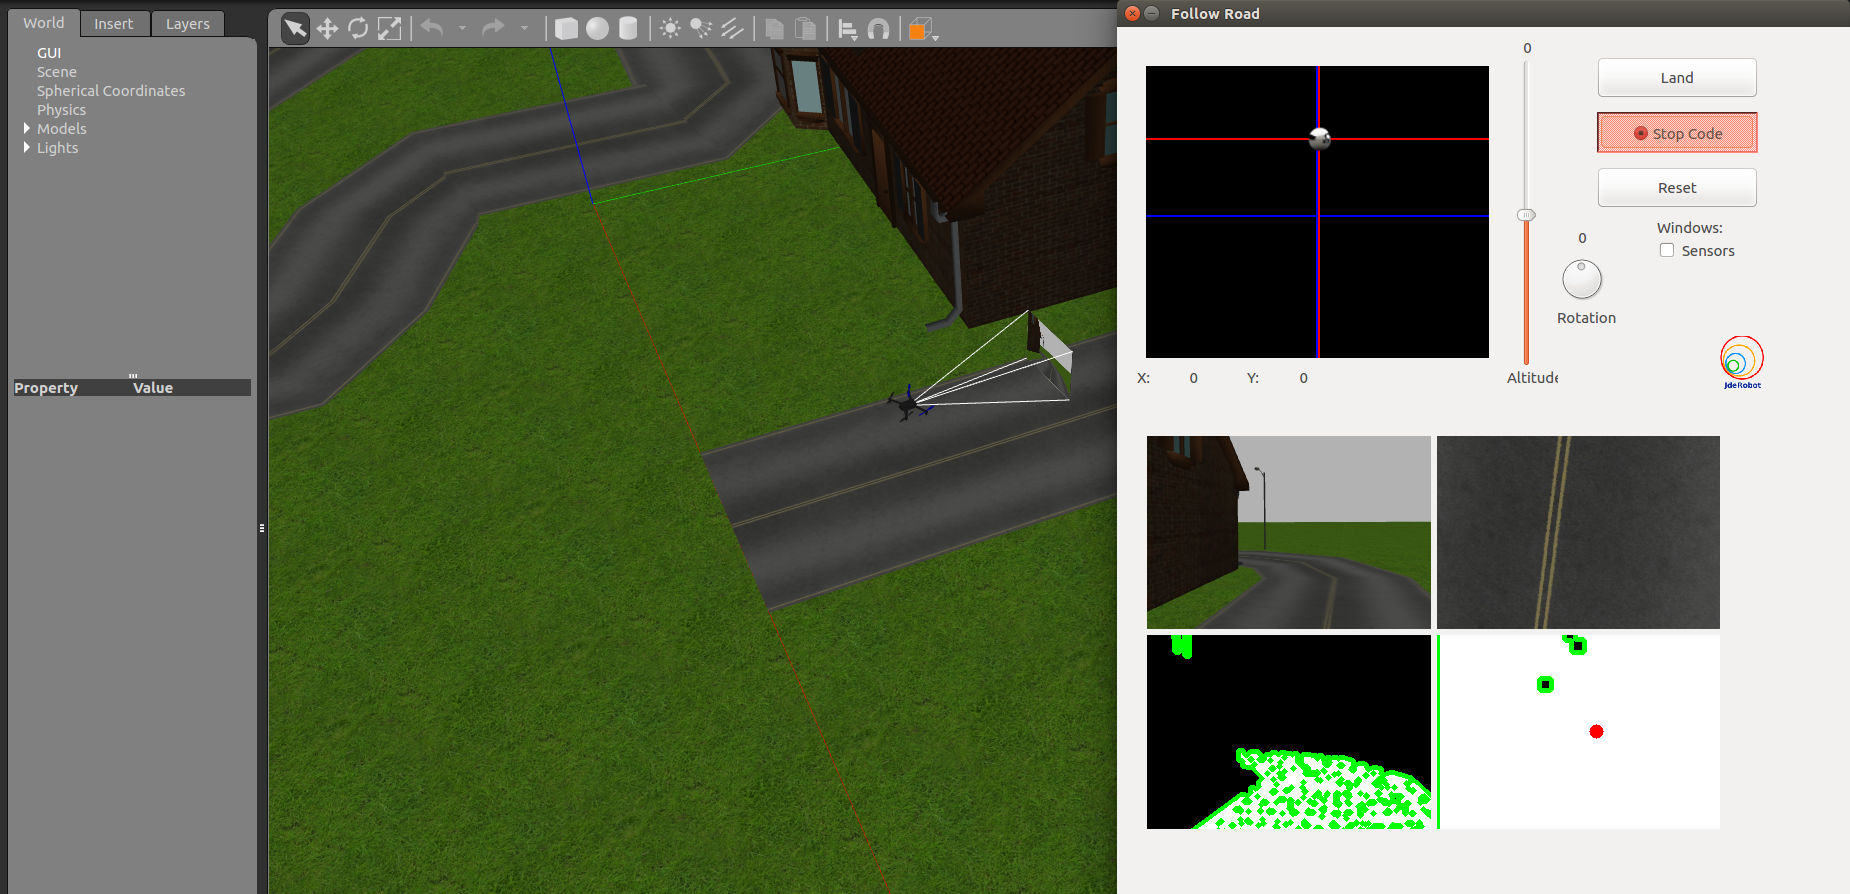
\includegraphics[width=0.98\textwidth]{figures/ejec_semiestat_fr.png}
		\caption{Ejecución con teleoperador}
		\label{fig.esefr}
		\end{center}
\end{figure}

Con esta ejecución semi-móvil de la práctica, el alumno también puede visualizar el comportamiento del robot al movimiento y el procesado dinámico de la imagen. Con esto, el alumno se puede hacer una idea de la velocidad a la que tiene que programar el control de movimiento para seguir la carretera.